\documentclass[11pt]{article}
\usepackage[margin=1in]{geometry}
\usepackage[utf8]{inputenc}
\usepackage[T1]{fontenc}
\usepackage{mathptmx,microtype,booktabs,graphicx,caption,enumitem,multirow,xcolor,amsmath}
\usepackage[most]{tcolorbox}
\usepackage[hidelinks]{hyperref}
\captionsetup{font=small,labelfont=bf}
\setlist{nosep,leftmargin=*}
\newcommand{\todo}[1]{\textcolor{red}{\textbf{[TODO: #1]}}}
\newcommand{\pct}[1]{#1\%}

\title{\textbf{Who Wrote It? Identifying LLM Families from Their Responses}\\[2pt]
\large CMPSC 448 Midterm Project}
\author{Team leader and sole member: \todo{Full name}\\
\small Code: \todo{GitHub repository URL}}
\date{October 2026}

\begin{document}
\maketitle

\begin{abstract}
We study whether the large language model (LLM) family behind a chatbot response can be identified from the text alone. Using 15{,}999 real single-turn conversations from the LMArena 140k release, balanced across eight families (Claude, DeepSeek, GPT, Gemini, Grok, Llama, Mistral, Qwen) and spanning 44 individual models, we train a character-level CNN and a word-level BiLSTM, alongside a TF-IDF baseline and a model that sees only 27 hand-crafted style features. The CNN reaches \pct{73.6} accuracy and TF-IDF \pct{74.8}, against \pct{12.5} chance (RQ1). The user's prompt carries no usable signal: input-only models stay at chance, which we trace to the Arena's prompt-independent model sampling (RQ2). Fingerprints transfer across task domains but lose up to 18 points, most on math (RQ3). Ablations show the signal is both structural and lexical: removing markdown, punctuation habits, whitespace layout, and length cuts accuracy from \pct{74} to \pct{53}, and a classifier using only 27 style statistics reaches \pct{61} (RQ4). Identifiability also varies sharply within families, from \pct{96} for o4-mini to \pct{37} for ChatGPT-4o.
\end{abstract}

%=====================================================================
\section{Problem Definition}
Given a response $y$ produced by an unknown LLM for a user prompt $x$, predict the family $f \in \mathcal{F}$ of the model that produced it, with $|\mathcal{F}| = 8$. Each example is a triple \texttt{(LLM\_name, LLM\_input, LLM\_output)}; we classify at the family level (e.g.\ \textit{Claude}) rather than the exact model version, since a family is the natural unit of ``who wrote it.'' We report accuracy and macro-F1 on a held-out test set; classes are balanced, so chance accuracy is $1/8 = \pct{12.5}$. We investigate all four research questions:
\begin{itemize}
  \item \textbf{RQ1}: How accurately can a CNN and an RNN identify the family from $y$ alone?
  \item \textbf{RQ2}: Does the prompt help? We compare $x$ only, $y$ only, and $(x, y)$.
  \item \textbf{RQ3}: Do fingerprints learned on some task domains transfer to an unseen domain?
  \item \textbf{RQ4}: Which characteristics (length, vocabulary, formatting, punctuation) distinguish the families, and how much does each contribute?
\end{itemize}

%=====================================================================
\section{Dataset Curation}
\subsection{Source}
We use \texttt{lmarena-ai/arena-human-preference-140k} \cite{chiang2024arena}, a public release of 135{,}634 ``battles'' from LMArena (formerly Chatbot Arena) collected between April 17 and July 25, 2025. In each battle a real user writes a prompt, two anonymous models answer it, and the user votes. Each row includes both conversations, the two model names, a timestamp, a language tag, an \texttt{is\_code} flag, and LMArena's automatic category tags (math, creative writing, instruction following, and others). The dataset is distributed under \todo{verify license on the Hugging Face dataset card; listed as CC-BY-4.0 by third-party catalogs}. We use it only for research, do not redistribute it, and do not add any private data. We chose this source over generating our own data because it is free, covers current frontier models, and contains real (not synthetic) user prompts.

\subsection{Construction pipeline (\texttt{prepare\_data.py})}
\begin{enumerate}
  \item \textbf{Filter}: keep English, single-turn conversations (one user turn, one assistant turn); prompts of 10 to 4{,}000 characters and responses of 50 to 8{,}000 characters; drop exact duplicates.
  \item \textbf{Map models to families} with name patterns (Table~\ref{tab:families}). Models outside the eight families (Gemma, Cohere Command, Amazon Nova, MiniMax, Kimi, Hunyuan) are dropped. Each side of a battle becomes its own row, so one prompt can yield two rows from different families.
  \item \textbf{Balance}: 95{,}408 rows remained (Claude 23{,}807 down to DeepSeek 5{,}369); we sample 2{,}000 per family uniformly at random, giving 16{,}000 rows.
  \item \textbf{Label domains} from the dataset's own tags, in priority order: \textit{code} (\texttt{is\_code}), \textit{math}, \textit{creative writing}, else \textit{general}. The domain mix is nearly identical across families (Table~\ref{tab:domains}), so domain cannot act as a shortcut for family.
\end{enumerate}

\begin{table}[htbp]
\centering\small
\caption{Families and the 44 models they contain (models listed by Arena name, version suffixes shortened).}
\label{tab:families}
\begin{tabular}{@{}lcp{11.2cm}@{}}
\toprule
Family & \# & Models \\ \midrule
Claude & 8 & opus-4, opus-4-thinking, sonnet-4, sonnet-4-thinking, 3.7-sonnet, 3.7-sonnet-thinking, 3.5-sonnet, 3.5-haiku \\
GPT & 8 & o3, o3-mini, o4-mini, chatgpt-4o-latest, gpt-4.1, gpt-4.1-mini, gpt-4o, gpt-4o-mini \\
Gemini & 8 & 2.5-pro (+2 previews), 2.5-flash (+1 preview), 2.5-flash-lite-thinking, 2.0-flash, 2.0-flash-thinking \\
Qwen & 6 & qwen3-235b (thinking, no-thinking, instruct-2507), qwen3-30b, qwen-max, qwq-32b \\
Grok & 4 & grok-3-preview, grok-3-mini-beta, grok-3-mini-high, grok-4 \\
Llama & 4 & llama-4-maverick (instruct, experimental), llama-4-scout, llama-3.3-70b \\
Mistral & 4 & mistral-medium, mistral-small (2506, 3.1-24b), magistral-medium \\
DeepSeek & 2 & deepseek-r1, deepseek-v3 \\ \bottomrule
\end{tabular}
\end{table}

\begin{table}[htbp]
\centering\small
\caption{Rows per family and domain after balancing (2{,}000 per family).}
\label{tab:domains}
\begin{tabular}{@{}lrrrrrrrr@{}}
\toprule
 & Claude & DeepSeek & GPT & Gemini & Grok & Llama & Mistral & Qwen \\ \midrule
code & 575 & 614 & 627 & 524 & 571 & 628 & 585 & 602 \\
general & 1175 & 1138 & 1093 & 1187 & 1120 & 1076 & 1149 & 1119 \\
creative writing & 151 & 152 & 157 & 152 & 181 & 157 & 162 & 158 \\
math & 99 & 96 & 123 & 137 & 128 & 139 & 104 & 121 \\ \bottomrule
\end{tabular}
\end{table}

\subsection{Preprocessing and leakage control (\texttt{src/preprocess.py})}
A classifier can score well for the wrong reasons, so we removed three shortcuts before training:
\begin{itemize}
  \item \textbf{Self-identification.} Responses such as ``I'm Claude, an AI assistant created by Anthropic'' make the task a name lookup. We replace model and vendor names (OpenAI, ChatGPT, GPT-$n$, Anthropic, Claude, Gemini, Bard, DeepMind, Llama, Meta AI, Qwen, DeepSeek, Mistral, Grok, xAI, and similar) with a \texttt{[MODEL]} token in both prompts and responses. A manual check of 25 random masked contexts found one false positive (``grok'' used as an English verb); the rest were genuine model or vendor names, including mentions in content (e.g.\ ``OpenAI Gym''), which we also want removed because which competitors a model mentions reflects its training cutoff. Masking reduces but does not eliminate the leak: the \emph{rate} of \texttt{[MODEL]} tokens still differs by family (Grok mentions itself most). Unmasked text is kept for an ablation (\S\ref{sec:rq4}).
  \item \textbf{Reasoning traces.} Visible \texttt{<think>} blocks would reveal reasoning models; we strip them. Only one response contained one, so this had no practical effect.
  \item \textbf{Prompt overlap across splits.} We split 70/15/15 \emph{grouped by prompt} (11{,}198 / 2{,}389 / 2{,}412 rows), so the two answers to one prompt never land in different splits. One near-empty response was dropped (15{,}999 rows).
\end{itemize}
We also flag rows for analysis: \textbf{reasoning variant} (by model name; from 0\% of Llama to 58\% of Grok), \textbf{refusal} (0.2\% to 3.2\%, highest for Claude), and \textbf{matched pair}, a prompt answered by two different families with both answers kept (2{,}301 rows, 371 in the test set). Matched pairs are the controlled subset for RQ2.

%=====================================================================
\section{Models and Training}
\subsection{Required models (\texttt{src/models.py})}
\textbf{CNN (character level).} Characters (the 300 most frequent symbols seen at least five times in training, plus padding, unknown, and separator tokens) are embedded in 64 dimensions. Three parallel 1D convolutions of widths 3, 5, and 7 (128 filters each) detect local patterns, following the multi-width design of \cite{kim2014cnn} applied to characters as in \cite{zhang2015charcnn}. Their outputs are concatenated (384 channels), batch-normalized, passed through ReLU and max-pooling by 2, then through a second width-5 convolution so that patterns spanning roughly 20 characters (e.g.\ a newline, a bullet marker, and bold text) can be detected. We pool globally with both max (``did this pattern occur?'') and mean (``how often?''), apply dropout 0.3, and classify with a linear layer. Input is the first 2{,}000 characters. Parameters: 888k. We chose characters because formatting (\texttt{**}, \texttt{\#\#\#}, newlines, dash variants) is invisible to most word tokenizers and was expected to be a strong signal.

\textbf{RNN (word level BiLSTM with attention).} Text is split into lowercased words, punctuation marks, and explicit newline tokens (vocabulary: the 30{,}000 most frequent tokens seen at least three times). Tokens are embedded in 128 dimensions and read by a one-layer bidirectional LSTM \cite{hochreiter1997lstm} with 128 hidden units per direction, using packed sequences so padding is ignored. Instead of using only the final state, an additive attention layer \cite{bahdanau2015attention} scores every position and pools a weighted sum, which lets the model focus on informative tokens anywhere in the response and lets us inspect what it attends to (\S\ref{sec:rq4}). Dropout 0.3, then a linear classifier. Input is the first 400 tokens. Parameters: 4.12M (3.84M of them in the embedding table).

\subsection{Baselines (\texttt{src/train.py})}
\textbf{TF-IDF + logistic regression}: word 1 to 2-grams (50k features, punctuation kept as tokens) and case-sensitive character 2 to 5-grams (100k features), sublinear TF, $C = 4$. \textbf{Stylometric GBM}: a gradient-boosted tree classifier on 27 hand-crafted features (length, average word and sentence length, type-token ratio over the first 200 words, rates of headers, bullets, bold, tables, horizontal rules, code fences, LaTeX, emoji, em and en dashes, curly quotes, exclamation and question marks, parentheses, first- and second-person pronouns, affirmation openers such as ``Great question!'', and closing offers such as ``Let me know if\ldots''). It sees no vocabulary, so it isolates structural signal. Both baselines train on the same training split.

\subsection{Training procedure}
\begin{table}[htbp]
\centering\small
\caption{Training configuration (identical for every experiment unless stated).}
\label{tab:hparams}
\begin{tabular}{@{}lll@{}}
\toprule
 & CNN & BiLSTM \\ \midrule
Input / max length & characters / 2{,}000 & words + punctuation / 400 \\
Optimizer & \multicolumn{2}{l}{AdamW, lr $10^{-3}$, weight decay $10^{-4}$, gradient clipping at norm 1.0} \\
Batch & \multicolumn{2}{l}{64, length-bucketed (sorted within chunks of 3{,}200, then shuffled) to minimize padding} \\
Schedule & \multicolumn{2}{l}{halve lr when validation macro-F1 stalls for 1 epoch} \\
Stopping & \multicolumn{2}{l}{max 20 epochs, early stop after 4 epochs without improvement; restore best checkpoint} \\
Loss & \multicolumn{2}{l}{cross-entropy (classes are balanced, so no weighting)} \\
Seeds & \multicolumn{2}{l}{3 (RQ1, RQ2), 1 (RQ3, RQ4); results reported as mean $\pm$ std across seeds} \\
Time per epoch & $\sim$24 s & $\sim$10 s \quad (\todo{GPU model}, PyTorch 2.5) \\ \bottomrule
\end{tabular}
\end{table}
Model selection uses only the validation split; the test split is touched once per trained model. Every finished run is cached by a hash of its configuration, seed, and exact data, so the pipeline resumes after interruptions and every number in this report can be regenerated with \texttt{python run\_all.py}. Figure~\ref{fig:curves} shows the training dynamics: the CNN's validation F1 keeps improving until epochs 9 to 16 and benefits from the learning-rate drops, while the BiLSTM's validation F1 levels off near 0.60 from about epoch 8 as its training loss keeps falling, a sign of overfitting that we return to in \S\ref{sec:depth}.

\begin{figure}[htbp]
\centering
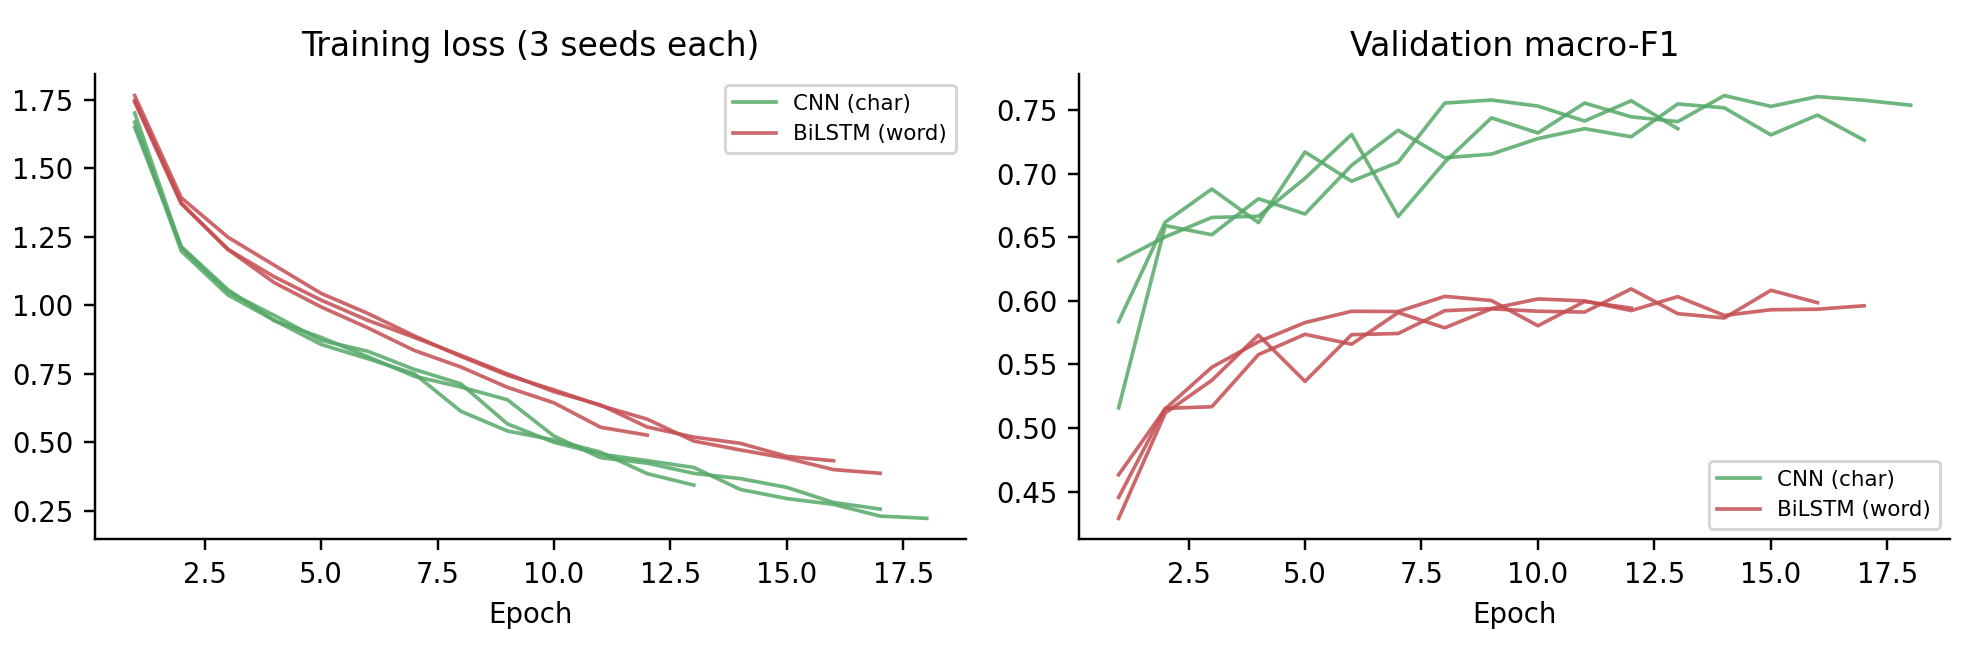
\includegraphics[width=0.85\linewidth]{figures/fig2_curves.png}
\caption{Training loss and validation macro-F1 for all three seeds of each model (RQ1).}
\label{fig:curves}
\end{figure}

%=====================================================================
\section{Results}
\subsection{RQ1: Identifying the family from the response}
\begin{table}[htbp]
\centering\small
\caption{RQ1 test results, output only (n = 2{,}412). Neural models: mean $\pm$ std over 3 seeds.}
\label{tab:rq1}
\begin{tabular}{@{}lccc@{}}
\toprule
Model & Accuracy (\%) & Macro-F1 (\%) & $\times$ chance \\ \midrule
Chance & 12.5 & 12.5 & 1.0 \\
Stylometric GBM (27 features) & 61.2 & 60.6 & 4.9 \\
BiLSTM (word) & 60.7 $\pm$ 1.2 & 59.8 $\pm$ 1.3 & 4.9 \\
CNN (char) & 73.6 $\pm$ 0.7 & 73.5 $\pm$ 0.7 & 5.9 \\
TF-IDF + logistic regression & \textbf{74.8} & \textbf{74.4} & 6.0 \\ \bottomrule
\end{tabular}
\end{table}

\begin{figure}[htbp]
\centering
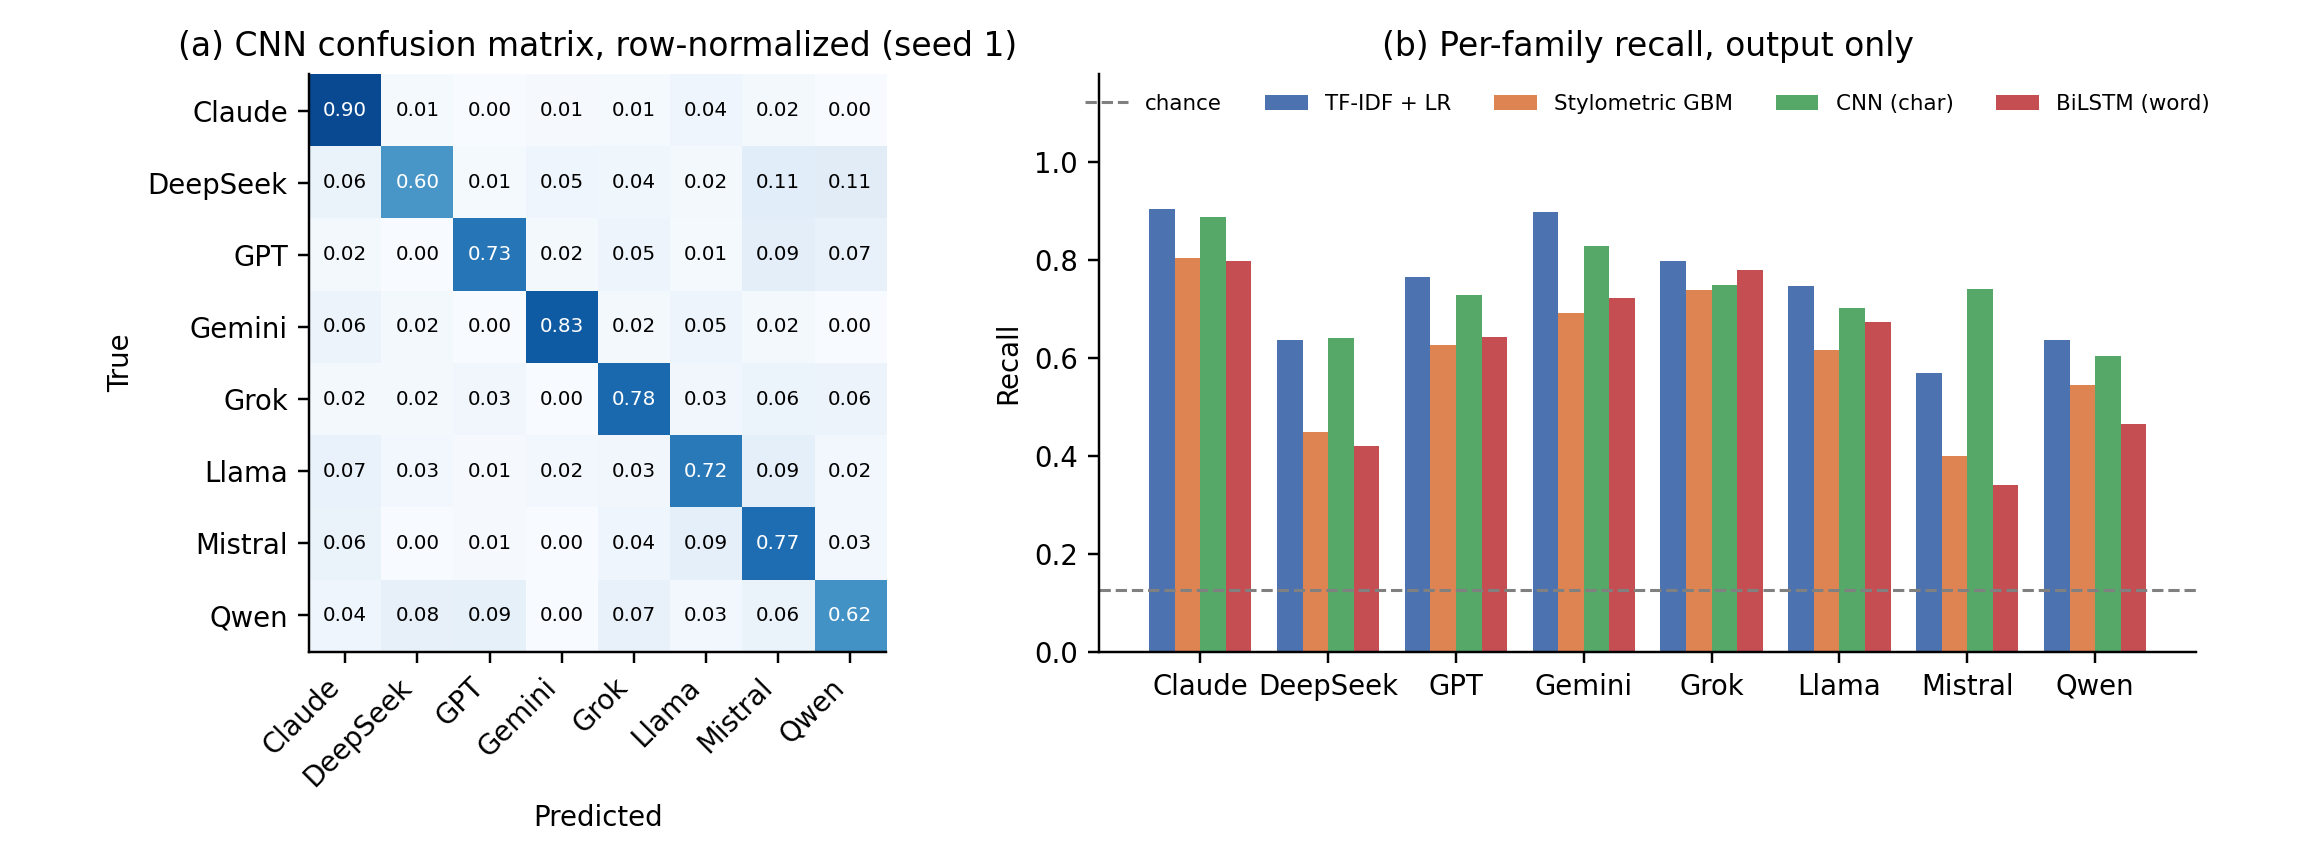
\includegraphics[width=\linewidth]{figures/fig1_rq1.png}
\caption{(a) Row-normalized confusion matrix of the best CNN seed (\pct{74.3}). (b) Per-family recall for all four models, averaged over seeds.}
\label{fig:rq1}
\end{figure}

\textbf{Yes, the family can be identified well above chance.} All models reach roughly 5 to 6 times chance (Table~\ref{tab:rq1}). The CNN (\pct{73.6}) and TF-IDF (\pct{74.8}) are close: the 1.2-point gap is under two seed standard deviations, so we treat them as comparable rather than claiming TF-IDF is better. With 11k training examples, a well-tuned n-gram model is a strong competitor for a neural model trained from scratch; this is a common result on small text-classification datasets. The BiLSTM is clearly weaker (\pct{60.7}); \S\ref{sec:depth} explains why.

\textbf{Some families are much easier than others} (Figure~\ref{fig:rq1}b). Claude (\pct{89} CNN recall) and Gemini (\pct{83}) are the most distinctive; Qwen (\pct{60}) and DeepSeek (\pct{64}) are the hardest. Errors are not random. Pooled over the three CNN seeds, the largest confusions are DeepSeek$\leftrightarrow$Qwen (\pct{10.6} and \pct{10.5} in each direction), GPT$\leftrightarrow$Qwen (\pct{9.3} and \pct{9.1}), and several families$\to$Mistral (\pct{8} to \pct{10}). TF-IDF's largest confusion is DeepSeek$\leftrightarrow$Mistral (\pct{12.6} and \pct{11.9}). These symmetric pairs suggest stylistically similar outputs; possible causes include similar post-training data or recipes, but our data cannot establish this.

%---------------------------------------------------------------------
\subsection{RQ2: Does the prompt help?}
\begin{table}[htbp]
\centering\small
\caption{RQ2 accuracy (\%) by input field. ``Matched'' is the subset of test prompts answered by two different families (n = 371), where an input-only model must give both rows the same label.}
\label{tab:rq2}
\begin{tabular}{@{}lcccccc@{}}
\toprule
 & \multicolumn{3}{c}{Full test set} & \multicolumn{3}{c}{Matched pairs} \\ \cmidrule(lr){2-4}\cmidrule(l){5-7}
Model & Input & Output & Both & Input & Output & Both \\ \midrule
TF-IDF + LR & 13.5 & 74.8 & 74.1 & 13.5 & 72.5 & 71.4 \\
CNN & 12.8 $\pm$ 0.2 & 73.6 $\pm$ 0.7 & 72.9 $\pm$ 0.4 & 11.0 $\pm$ 0.5 & 74.4 $\pm$ 0.2 & 73.1 $\pm$ 0.5 \\
BiLSTM & 12.7 $\pm$ 0.5 & 60.7 $\pm$ 1.2 & 60.2 $\pm$ 1.7 & 12.2 $\pm$ 1.1 & 58.9 $\pm$ 2.6 & 58.0 $\pm$ 3.3 \\
\midrule
Timestamp only (GBM) & \multicolumn{3}{c}{19.4} & \multicolumn{3}{c}{16.4} \\ \bottomrule
\end{tabular}
\end{table}

\begin{figure}[htbp]
\centering
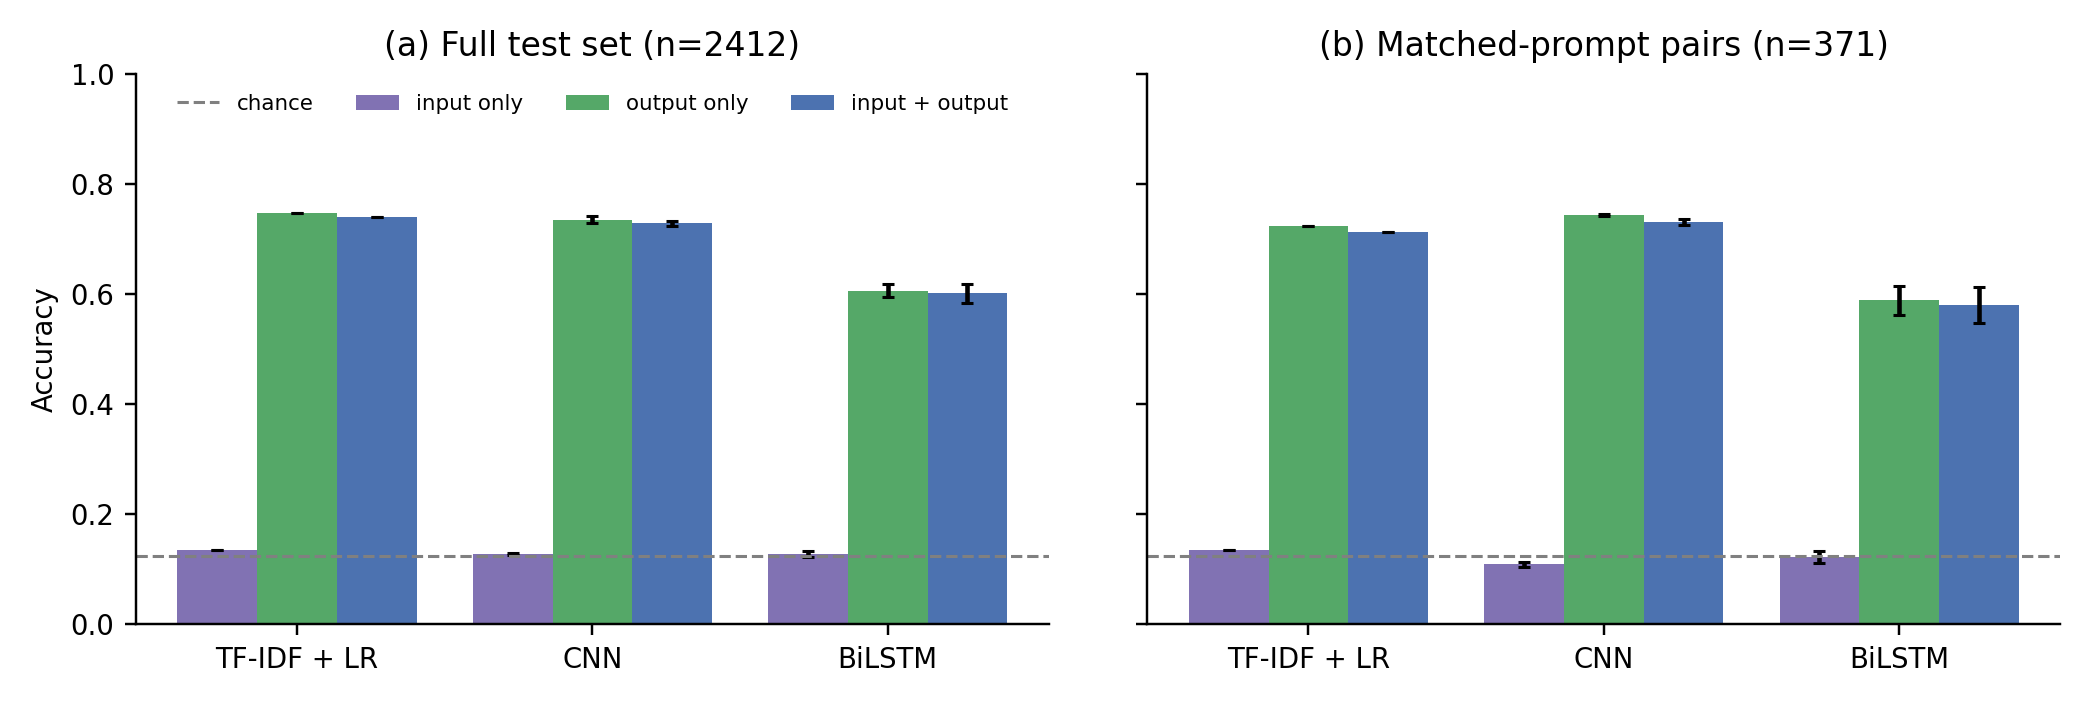
\includegraphics[width=0.92\linewidth]{figures/fig3_rq2.png}
\caption{RQ2: accuracy by input field on the full test set and on matched-prompt pairs. Error bars: std over 3 seeds.}
\label{fig:rq2}
\end{figure}

\textbf{(i) The LLM cannot be predicted from the prompt.} Input-only accuracy is 12.7 to \pct{13.5} for all three models, statistically indistinguishable from chance (one-sided binomial test against 12.5\%: $p = 0.07$ for TF-IDF, $p = 0.35$ for the CNN). The top-weighted input n-grams per family are generic words (``summer'', ``national'', ``bear'') with no coherent pattern, the signature of a model fitting noise.

\textbf{(ii) Adding the prompt does not improve classification}; it slightly hurts (by 0.5 to 0.7 points). For the neural models the prompt takes a quarter of the sequence budget that would otherwise hold response text, and for all models it adds features unrelated to the label.

\textbf{(iii) Why input-only fails here, and when it would work.} We initially expected input-only to beat chance through a temporal confound: models enter and leave the Arena at different times, and prompt topics drift. That effect exists but is weak. A classifier given only the timestamp reaches \pct{19.4}, mostly by recognizing families whose availability window differs (Mistral, whose first response is May 17 versus April 17 to 25 for the others, has \pct{37} timestamp-only recall). Over a three-month window, though, the drift in \emph{what users ask} is too small to detect with 11k examples. The deeper reason is the data-generating process: on LMArena the user writes the prompt before knowing which models will answer, and the pair is sampled independently of the prompt, so $x$ and $f$ are close to independent by design. Input-only classification would ``work surprisingly well'' on datasets where this independence is broken, for example when each model was run on a different benchmark, when users choose which model to ask (so prompt style reflects the model's user base), or when prompts mention the model by name (1.2 to \pct{2.0} of our prompts do, and these are masked). A high input-only score is therefore a diagnostic for dataset construction bias, not evidence of a model fingerprint.

The matched-pair results confirm that the output classifiers are not exploiting prompt content: on prompts answered by two different families, the CNN's output-only accuracy (\pct{74.4}) is the same as on the full set.

%---------------------------------------------------------------------
\subsection{RQ3: Do fingerprints generalize across domains?}
For each target domain $D$ we hold out \pct{30} of $D$'s prompts as the test set and train two models evaluated on \emph{exactly the same test rows}: an \emph{in-domain} model trained on the rest of $D$, and a \emph{cross-domain} model trained only on other domains, subsampled to the same size and kept family-balanced. Matching the training size matters: without it, a cross-domain drop could simply reflect a different amount of training data.

\begin{table}[htbp]
\centering\small
\caption{RQ3 accuracy (\%) on each target domain's test set: in-domain / cross-domain (drop). Single seed.}
\label{tab:rq3}
\begin{tabular}{@{}lrrccc@{}}
\toprule
Target domain & $n_\text{train}$ & $n_\text{test}$ & TF-IDF + LR & CNN & BiLSTM \\ \midrule
code & 3{,}307 & 1{,}419 & 70.4 / 65.5 ($-$4.9) & 69.1 / 58.5 ($-$10.6) & 56.8 / 46.7 ($-$10.1) \\
general & 6{,}344 & 2{,}713 & 74.8 / 70.4 ($-$4.4) & 72.5 / 72.0 ($-$0.5) & 58.1 / 54.9 ($-$3.2) \\
creative writing & 876 & 394 & 58.4 / 51.0 ($-$7.4) & 54.3 / 44.2 ($-$10.2) & 31.5 / 31.2 ($-$0.3) \\
math & 665 & 281 & 62.3 / 50.2 ($-$12.1) & 59.8 / 46.3 ($-$13.5) & 48.0 / 30.2 ($-$17.8) \\ \bottomrule
\end{tabular}
\end{table}

\begin{figure}[htbp]
\centering
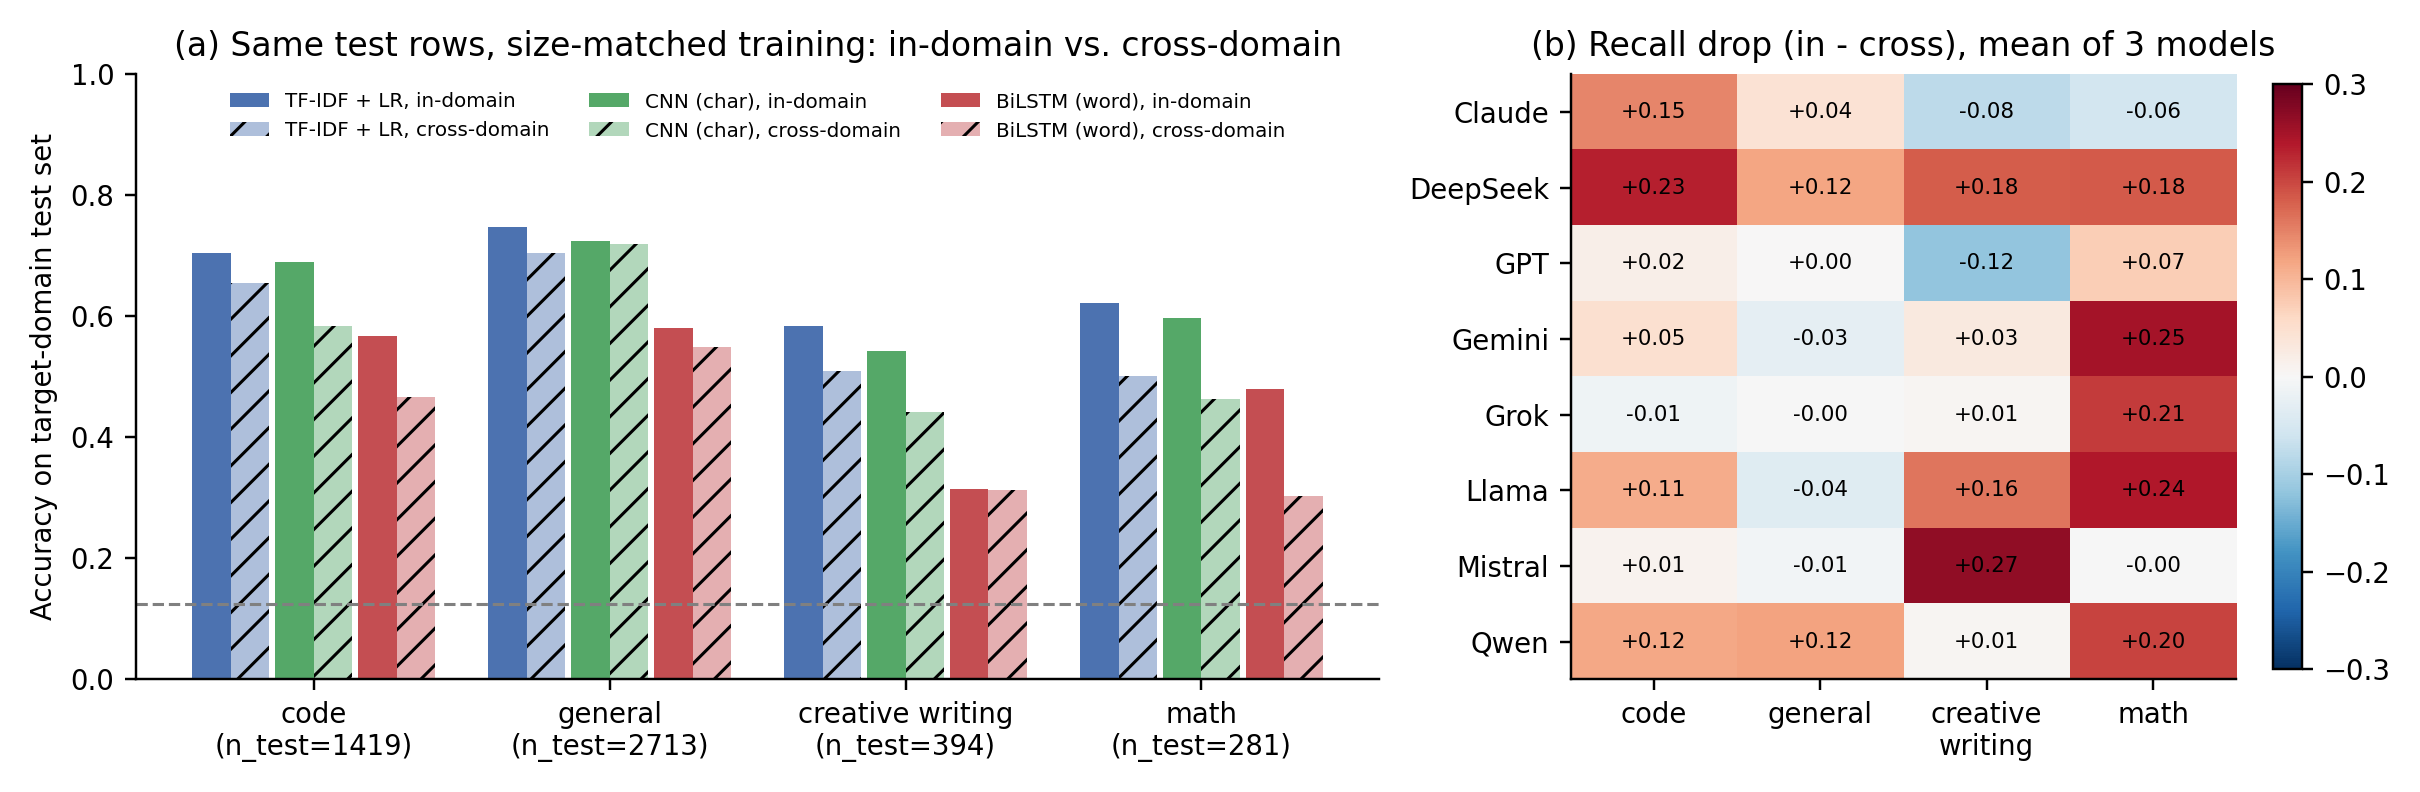
\includegraphics[width=\linewidth]{figures/fig4_rq3.png}
\caption{RQ3. (a) In-domain (solid) vs.\ cross-domain (hatched) accuracy on identical test rows. (b) Per-family recall drop under domain shift, averaged over the three models; red means the family is harder to recognize on an unseen domain.}
\label{fig:rq3}
\end{figure}

\textbf{(i) Performance decreases on unseen domains, but most of the fingerprint survives.} Cross-domain accuracy stays 2.4 to 5.8 times above chance in every case, so the classifiers are not purely task-specific. The size of the drop depends on how different the target domain is: transferring into \emph{general} costs the CNN half a point (general prompts are the most similar to the mixture of the other domains), while \emph{code} and \emph{math} cost 10 to 14 points. Math is consistently the hardest transfer for all models. Math answers are dominated by equations and step-by-step derivations, a format that crowds out the stylistic habits (openers, closing offers, prose formatting) that the classifiers learn elsewhere. The creative-writing and math test sets are small (394 and 281 rows, so the standard error of each accuracy is about 2.5 to 3 points) and use a single seed, so differences of a few points there should not be over-interpreted.

\textbf{(ii) Some families are more consistently identifiable} (Figure~\ref{fig:rq3}b). GPT, Grok, and Mistral lose almost nothing on code and general text; DeepSeek loses 12 to 23 points of recall on every domain, making its fingerprint the most task-specific. Gemini, Grok, Llama, and Qwen all drop 20 to 25 points on math specifically. Mistral's 27-point drop on creative writing is the largest single cell but rests on about 49 test rows.

\textbf{(iii) General fingerprint or task-specific pattern?} Both. A substantial, domain-independent component exists (cross-domain accuracy far above chance), and a task-specific component adds 5 to 14 points when training data matches the target domain. The CNN, which relies most on formatting (\S\ref{sec:rq4}), transfers worst into code, where formatting is dictated by the code itself; TF-IDF, which also uses vocabulary, transfers into code better ($-$4.9 vs.\ $-$10.6).

%---------------------------------------------------------------------
\subsection{RQ4: What distinguishes the families?}
\label{sec:rq4}
\textbf{Family profiles.} Figure~\ref{fig:rq4profile}a shows family means of selected style features. Each family has a recognizable house style:
\begin{itemize}
  \item \textbf{Claude} writes the shortest answers (median 180 words versus 349 to 593 for the others), uses the least bold text, prefers hyphen bullets, and essentially never uses typographic (curly) quotes (0.00 per 1k characters).
  \item \textbf{GPT} uses the most curly quotes (3.19 per 1k characters), the most em dashes and tables, round bullet characters, and frequent horizontal rules.
  \item \textbf{Gemini} opens with an affirmation (``Okay,'' ``Of course'') in \pct{41} of responses versus at most \pct{17} for any other family, and almost never ends by offering further help (\pct{3}).
  \item \textbf{Qwen} uses the most horizontal rules (4.1 per response), the most headers and emoji, including check-mark emoji in lists.
  \item \textbf{DeepSeek} uses the most bold text (5.6 bold spans per 100 words), followed by Qwen and Mistral (4.8); Mistral most often closes by offering more help (``Would you like\ldots'', \pct{38} of responses).
  \item \textbf{Llama} has the lowest lexical diversity (type-token ratio 0.57 versus 0.60 to 0.66) and favors numbered lists with bolded items.
  \item \textbf{Grok} writes the longest answers (median 593 words) and uses connective phrasing (``such as,'' ``if you'').
\end{itemize}
The top TF-IDF n-grams and the BiLSTM's attention agree with these profiles. For example, the BiLSTM gives the token ``okay'' 160 times the average attention weight in Gemini responses, and curly quote characters 31 to 41 times the average in GPT responses.

\begin{figure}[htbp]
\centering
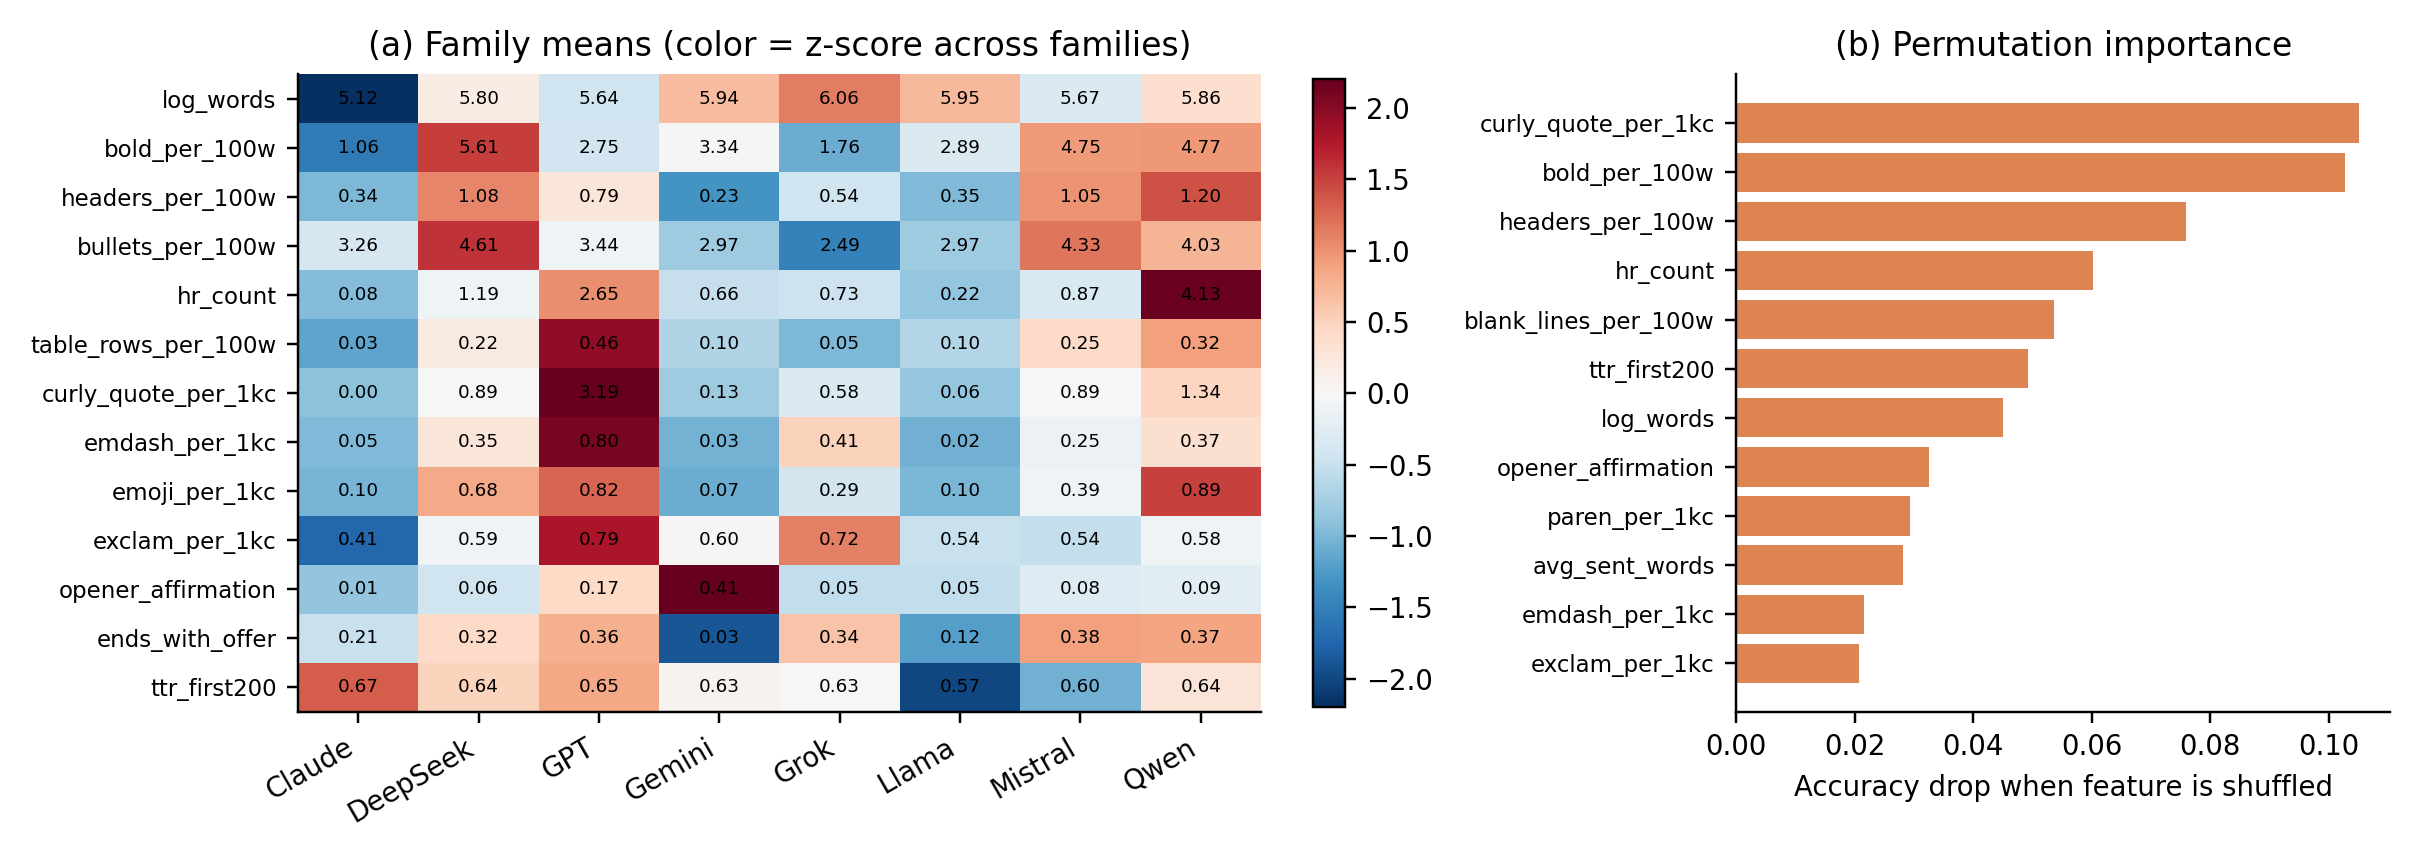
\includegraphics[width=\linewidth]{figures/fig5_rq4_profile.png}
\caption{RQ4. (a) Family means of selected style features; cell text is the raw mean, color is the z-score across families. (b) Permutation importance of the stylometric GBM's features (accuracy lost when one feature is shuffled).}
\label{fig:rq4profile}
\end{figure}

\textbf{(i) Which signals does the classifier use?} The structure-only GBM reaches \pct{61.2} with no access to vocabulary. Its most important features (Figure~\ref{fig:rq4profile}b) are curly-quote rate, bold rate, header rate, horizontal rules, blank-line rate, lexical diversity, and length. These are typography and layout decisions, not content.

\begin{figure}[htbp]
\centering
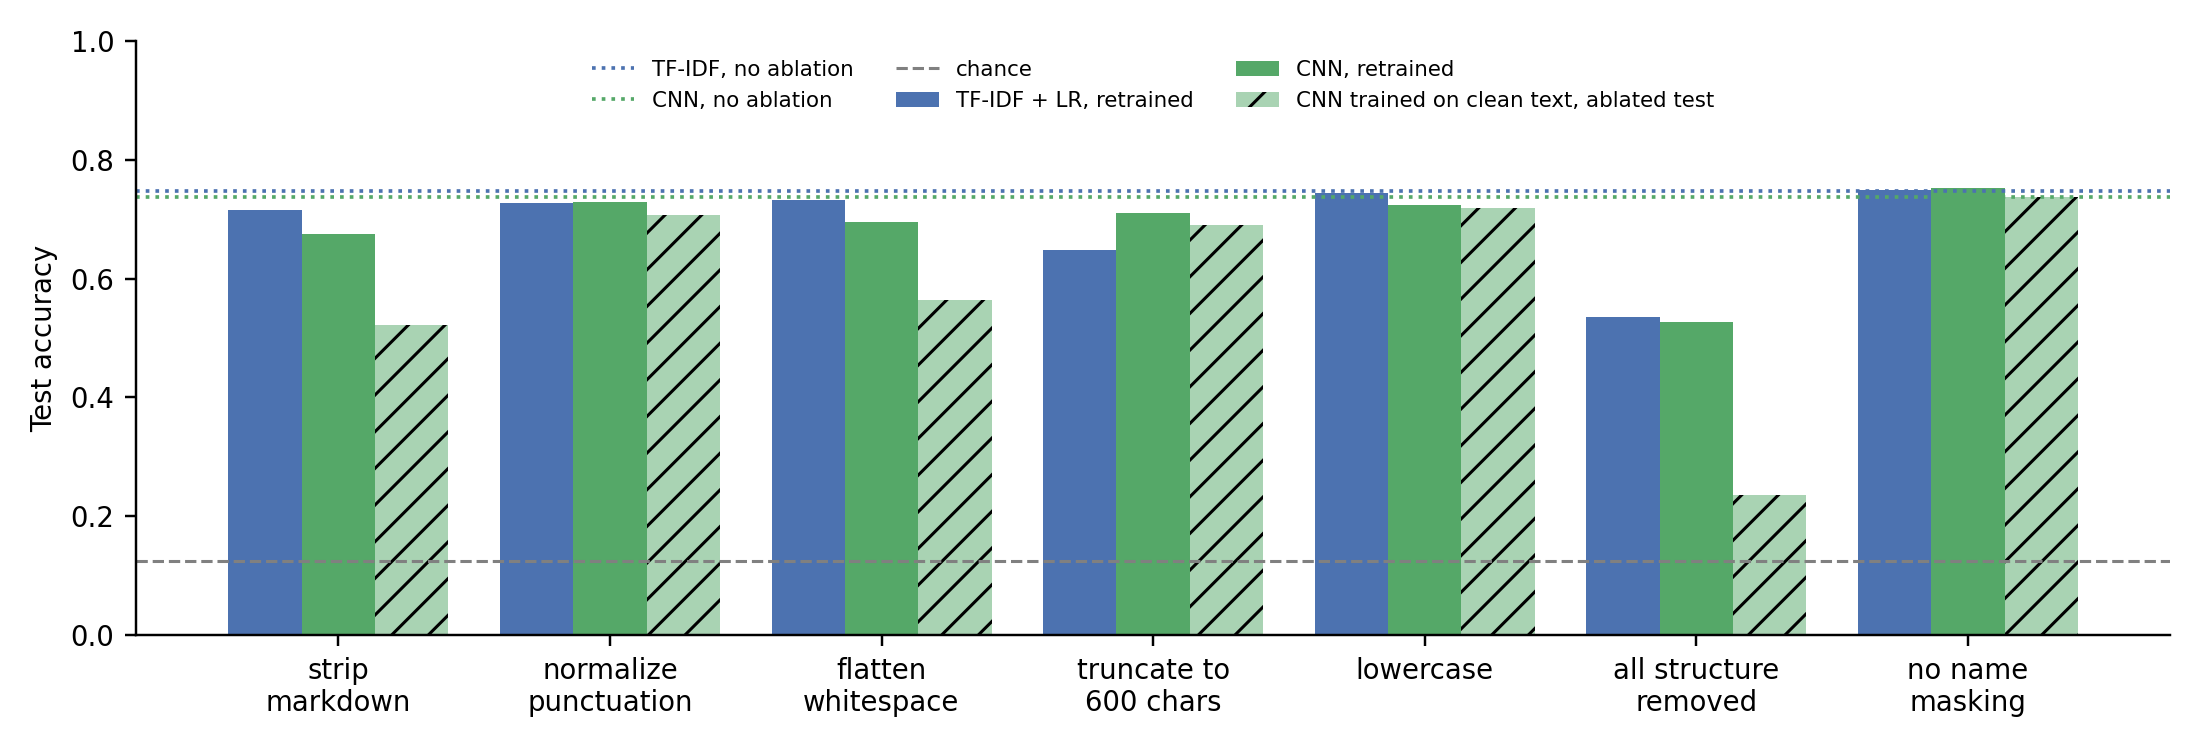
\includegraphics[width=\linewidth]{figures/fig6_rq4_ablation.png}
\caption{RQ4 ablations. Solid bars: retrain and test on transformed text (is the information needed?). Hatched: the CNN trained on clean text, tested on transformed text (does the trained model rely on it?). Dotted lines: unablated accuracy.}
\label{fig:ablation}
\end{figure}

\textbf{(ii, iii) Linguistic, structural, or both? Ablations.} We transform the text to remove one kind of signal and measure accuracy in two ways (Figure~\ref{fig:ablation}, Table~\ref{tab:ablation}): \emph{retraining} on transformed text measures whether the information is needed at all, while testing the \emph{clean-trained} CNN on transformed text measures whether that model relies on it.

\begin{table}[htbp]
\centering\small
\caption{RQ4 ablation accuracy (\%). ``All structure removed'' applies markdown stripping, punctuation normalization, whitespace flattening, truncation to 600 characters, and lowercasing together.}
\label{tab:ablation}
\begin{tabular}{@{}lccc@{}}
\toprule
Transformation & TF-IDF (retrained) & CNN (retrained) & CNN (clean model) \\ \midrule
None & 74.8 & 73.7 & 73.7 \\
Strip markdown (headers, bullets, bold, tables, rules) & 71.5 & 67.5 & 52.2 \\
Normalize punctuation (dashes, curly quotes, emoji) & 72.7 & 72.9 & 70.6 \\
Flatten whitespace (all newlines to spaces) & 73.3 & 69.5 & 56.4 \\
Truncate to 600 characters (removes length) & 64.8 & 71.0 & 68.9 \\
Lowercase & 74.5 & 72.4 & 71.9 \\
All structure removed & 53.5 & 52.7 & 23.6 \\
No name masking (self-identification left in) & 74.9 & 75.2 & 73.7 \\ \bottomrule
\end{tabular}
\end{table}

Three conclusions follow:
\begin{enumerate}
  \item \textbf{Both kinds of signal matter.} Removing all structure costs about 21 points (74 to 53), so structure is a major component. But \pct{53} remains with only lowercased, unformatted, truncated word content, which is still 4 times chance. Combined with the structure-only GBM's \pct{61}, neither signal alone explains the full \pct{74}. This agrees with \cite{sun2025idiosyncrasies}, who find model idiosyncrasies persist in word-level distributions.
  \item \textbf{The CNN depends heavily on layout but the signal is redundant.} Stripping markdown drops the clean-trained CNN from 73.7 to \pct{52.2}, and removing all structure drops it to \pct{23.6}; yet retraining on the same text recovers 67.5 and \pct{52.7}. The trained model chooses the easiest cues, but other cues are available when those are taken away.
  \item \textbf{Length matters most to TF-IDF} ($-$10.0 when truncated to 600 characters versus $-$2.7 for the CNN, which already sees at most 2{,}000 characters). Longer responses contain more evidence: TF-IDF accuracy rises from \pct{65.2} on the shortest quarter of responses to \pct{81.6} on the longest.
\end{enumerate}
\textbf{Self-identification is not driving our results.} Removing the name masking improves accuracy by only 0.1 (TF-IDF) to 1.5 (CNN) points, consistent with only 0.8 to \pct{6.9} of responses mentioning their own family.

%=====================================================================
\section{Further Analyses}
\label{sec:depth}
\textbf{Fingerprints are per model, not per family.} Accuracy varies more within some families than between families (best CNN seed, test set; $n$ in parentheses):
\begin{itemize}
  \item GPT: o4-mini \pct{96} (48), o3 \pct{87} (54), gpt-4.1 \pct{79} (42), but chatgpt-4o-latest \pct{37} (51).
  \item Grok: grok-3-mini-high \pct{95} (56) and grok-4 \pct{95} (20), but grok-3-preview \pct{44} (88).
  \item Mistral: mistral-small-2506 \pct{91} (34) and mistral-medium \pct{85} (149), but the reasoning model magistral-medium only \pct{41} (32).
  \item Qwen: qwen3-30b \pct{78} (54), but qwen3-235b without thinking \pct{50} (92).
  \item Claude is the exception: every one of its eight models scores 82 to \pct{95}.
\end{itemize}
A ``family'' is therefore an abstraction over models that can write quite differently. Claude's consistency across versions explains why it is the easiest family; GPT's and Grok's internal diversity explains part of their confusion with others. A natural follow-up would be to classify individual models directly.

\textbf{Reasoning variants are easier to identify} (TF-IDF \pct{79.7} vs.\ \pct{72.3}; CNN \pct{78.5} vs.\ \pct{72.2}). We treat this cautiously because the share of reasoning variants differs by family (0\% of Llama, 58\% of Grok), so this comparison is confounded with family identity; the per-model results above show that some reasoning models (o4-mini) are highly identifiable while others (magistral) are not.

\textbf{TF-IDF and the CNN make different errors.} Each is about \pct{74} accurate, yet they agree on only \pct{71} of test predictions (two CNN seeds agree with each other on 82 to \pct{86}). Since each model is right on only about three-quarters of the rows, this level of disagreement implies that a substantial share of rows is classified correctly by one model but not the other. This makes them good candidates for an ensemble, which we leave to future work.

\textbf{Why the BiLSTM underperforms.} Three design factors combine. (1) \emph{Overfitting}: 3.84M of its 4.12M parameters are word embeddings learned from only 11k documents, and its validation F1 stops improving around epoch 8 while training loss keeps falling (Figure~\ref{fig:curves}). (2) \emph{Lossy view of formatting}: word tokenization discards spaces and indentation, splits \texttt{**} into two separate asterisks, and lowercases text, which weakens exactly the layout cues the ablations show are most useful. (3) \emph{Truncation}: 400 tokens cover less of a long response than the CNN's 2{,}000 characters do for formatting-dense text. Its attention weights confirm it learned to look at the same cues (curly quotes, \texttt{\#}, em dashes, ``okay''), but through a coarser representation. Character-level input or subword tokens with smaller embeddings would likely close part of the gap.

\textbf{Refusals are harder} (CNN \pct{55} on refusals vs.\ \pct{75} otherwise; about 30 test rows): refusals are short and formulaic, leaving little room for style.

%=====================================================================
\section{Limitations}
\begin{itemize}
  \item \textbf{Uncontrolled generation.} We do not know each model's system prompt, temperature, or the Arena's serving pipeline. Some typographic signals (for example curly quotes) could come from post-processing rather than the model itself.
  \item \textbf{Family heterogeneity.} Families contain 2 to 8 models in unequal proportions, so family accuracy partly reflects which versions were sampled.
  \item \textbf{Single seed for RQ3 and RQ4}, and small creative-writing and math test sets.
  \item \textbf{Regex masking} has rare false positives and leaves the \texttt{[MODEL]} token frequency as a residual signal.
  \item \textbf{Snapshot in time.} The data covers April to July 2025 models only, in English only; fingerprints change as models are updated.
\end{itemize}

%=====================================================================
\section{Lessons and Experience}
\begin{tcolorbox}[colback=red!4,colframe=red!60,title=\textbf{TODO: write this section yourself (20\% of the grade)}]
\small Write 1 to 1.5 pages in your own words. Concrete, specific lessons score better than general statements. Things that actually happened in this project, to choose from and expand:
\begin{itemize}
  \item The initial RQ2 hypothesis (input-only would beat chance via a temporal confound) was wrong. What did testing it teach you about how a dataset's collection process determines what is learnable?
  \item A TF-IDF baseline matched the CNN. When is a simple baseline the right first step, and what would you do with more data?
  \item The 12-epoch cap left the CNN under-trained; reading the validation curves revealed it.
  \item The first full run was lost to the laptop sleeping and restarting; the timing logs revealed it, and run caching made the pipeline resumable.
  \item Masking self-identification by regex was imperfect (``grok'' as a verb, residual token frequency).
  \item Within-family differences were larger than expected; ``family'' turned out to be a leaky label.
  \item Constraints (no budget for API calls) pushed the project to Arena data, which changed what RQ2 could show.
  \item What you would do differently with another week.
\end{itemize}
Delete this box when done.
\end{tcolorbox}

%=====================================================================
\section{Reproducibility}
All code is in the repository. \texttt{python prepare\_data.py} downloads and builds the dataset; \texttt{python run\_all.py} runs preprocessing and all four research questions; \texttt{python report/make\_figures.py} rebuilds the report figures from \texttt{results/*.json}. Every run is seeded and cached by a hash of its configuration and data.

\begin{thebibliography}{9}\small
\bibitem{chiang2024arena} W.-L. Chiang, L. Zheng, Y. Sheng, et al. Chatbot Arena: An open platform for evaluating LLMs by human preference. \textit{ICML}, 2024.
\bibitem{sun2025idiosyncrasies} M. Sun, Y. Yin, Z. Xu, J. Z. Kolter, Z. Liu. Idiosyncrasies in large language models. \textit{ICML}, 2025.
\bibitem{kim2014cnn} Y. Kim. Convolutional neural networks for sentence classification. \textit{EMNLP}, 2014.
\bibitem{zhang2015charcnn} X. Zhang, J. Zhao, Y. LeCun. Character-level convolutional networks for text classification. \textit{NeurIPS}, 2015.
\bibitem{hochreiter1997lstm} S. Hochreiter, J. Schmidhuber. Long short-term memory. \textit{Neural Computation}, 9(8):1735--1780, 1997.
\bibitem{bahdanau2015attention} D. Bahdanau, K. Cho, Y. Bengio. Neural machine translation by jointly learning to align and translate. \textit{ICLR}, 2015.
\end{thebibliography}
\end{document}
